\documentclass[10pt,a4paper]{report}
\usepackage[utf8]{inputenc}
\usepackage[spanish]{babel}
\usepackage{amsmath}
\usepackage{amsfonts}
\usepackage{amssymb}
\usepackage{makeidx}
\usepackage{graphicx}
\usepackage{titlesec}
\usepackage{sectsty}
\usepackage{listings}
\usepackage{color}
\usepackage{float}
\usepackage{hyperref}
\usepackage{apacite}

\titleformat{\chapter}[display]
{\normalfont\bfseries}{}{0pt}{\Large}
\chaptertitlefont{\Huge}

\definecolor{codegreen}{rgb}{0,0.6,0}
\definecolor{codegray}{rgb}{0.5,0.5,0.5}
\definecolor{codepurple}{rgb}{0.58,0,0.82}
\definecolor{backcolour}{rgb}{0.95,0.95,0.92}

\lstdefinestyle{mystyle}{
	backgroundcolor=\color{backcolour},   
	commentstyle=\color{codegreen},
	keywordstyle=\color{magenta},
	numberstyle=\tiny\color{codegray},
	stringstyle=\color{codepurple},
	basicstyle=\footnotesize,
	breakatwhitespace=false,         
	breaklines=true,                 
	captionpos=b,                    
	keepspaces=true,                 
	numbers=left,                    
	numbersep=5pt,                  
	showspaces=false,                
	showstringspaces=false,
	showtabs=false,                  
	tabsize=2,
	frame=lines
}

\lstset{style=mystyle}

\author{Medina Medina, David A.\\
	Benlliure Jiménez, Mº Cristina\\
	Brito Ramos, Christian\\
	López González, Néstor\\\\
	Dr. Modesto Fernando Castrillon Santana}
\title{Práctica 9 - Programación del LED integrado}
\begin{document}
	\maketitle
	\tableofcontents
	\bibliographystyle{apacite}
	\chapter{Introducción}
	\textit{Arduino} es el primer proyecto de hardware en open-source que facilita el diseño de productos digitales que requieren de un microcontrolador.
	
	El objetivo de este proyecto \cite{repositorio-github} consiste en utilizar la placa \textit{Arduino UNO R3} para controlar la frecuencia de parpadeo del LED integrado en la placa, de modo que, la frecuencia de parpadeo sea mayor cuanto más positivo sea el valor de la onda portadora senoidal.
	
	
	\chapter{Método y materiales}
	\section{Materiales}
	El desarrollo de este proyecto se ha llevado a cabo utilizando el IDE de desarrollo de aplicaciones \textit{C/C++} de \textit{JetBrains}, \textit{CLion}, y las siguientes herramientas:
	\begin{itemize}
		\item Placa Arduino Uno R3.
		\item Librería \texttt{Arduino.h} \cite{arduino-reference}.
		\item Archivo \texttt{CMakeLists.txt} para la construcción automatizada de las dependencias de la librería \texttt{Arduino.h}.
	\end{itemize}

	El proyecto también puede cargarse en la placa usando el el IDE oficial de \textit{Arduino}.  
	
	\section{Método}
	El código que se cargará en la placa se encuentra el el archivo \texttt{Practica9.ino} el cual se estructura en las siguientes partes:
	\begin{itemize}
		\item Macros y variables globales
		\item Rutina \texttt{setup()}.
		\item Rutina \texttt{loop()}.
	\end{itemize}
	
	
	\subsection{Macros y variables globales}
	En primer lugar, se incluye la librería \texttt{Arduino.h} que contiene todas las rutinas primitivas que utilizaremos para comunicarnos con la placa.
	
	Se declaran un conjunto de macros que serán utilizadas en el código:
	\begin{description}
		\item[\texttt{AMPLITUDE}] Esta macro contiene el valor de la amplitud de la onda sinusoidal que generaremos. Por defecto, su valor es igual a 1 unidad.
		\item[\texttt{MIN\_FREQ}] Se establece el valor de la frecuencia de la onda senoidal. Por defecto: 1 Hz.
		\item[Rutina \texttt{sine\_wave(f, t)}] Esta macro define una rutina que tomará como parámetro de entrada una frecuencia, \texttt{f}, y una magnitud de tiempo, \texttt{t}. La onda senoidal generada esta definida por esta ecuación,
		
		\begin{equation*}
			s(f,t) = A \sin ( 2 \pi f t )
		\end{equation*}
		
		donde $A$ es la amplitud de onda, $f$ es la frecuencia y $t$ el tiempo.
	\end{description}
	
	En último lugar se inicializa una variable global a 0 (\texttt{clockTick}). Esta variable incrementa su valor en una unidad en cada iteración de la rutina \texttt{loop()} para poder extraer el valor de la onda senoidal generada en un tick de tiempo determinado. 
	
	\lstinputlisting[language=C++, firstline=1, lastline=7]{../src/Practica9.ino}
	
	\subsection{Rutina \texttt{setup()}}
	Esta primitiva realiza los ajustes iniciales de la placa. Se establece la velocidad de transmisión de datos de la placa a 9600 baudios y se configura el pin número 13 (definido por la macro primitiva \texttt{LED\_BUILTIN}) como pin de salida.
	
	\lstinputlisting[language=C++, firstline=9, lastline=12]{../src/Practica9.ino}
	
	\subsection{Rutina \texttt{loop()}}
	Esta rutina primitiva define el bucle principal que se ejecuta en la placa \textit{Arduino}. 
	
	En la variable \texttt{s} se guarda el valor de la función sinusoidal con frecuencia mínima, \texttt{FREQ\_MIN}, y un tiempo, \texttt{clockTick}.
	
	La frecuencia de parpadeo se especifica en la variable \texttt{f}, donde la frecuencia variará su valor en el rango $\left[ MIN\_FREQ, 2 \times MIN\_FREQ \right]$ determinado por la siguiente fórmula,
	
	\begin{equation*}
		f = MIN\_FREQ + MIN\_FREQ(s / AMPLITUDE) + MIN\_FREQ
	\end{equation*}
	
	donde $MIN\_FREQ$ es la frecuencia mínima de oscilación del LED --coincide con la frecuencia de la onda senoidal generada--, $s$ es el valor de la onda sinusoidal para un tick de tiempo determinado y $AMPLITUDE$ es la amplitud máxima de la onda generada.
	
	A continuación, se define en la variable \texttt{t} el periodo en segundos de parpadeo del LED con la siguiente ecuación,
	
	\begin{equation*}
	t = 1 / f
	\end{equation*}
	
	donde $t$ es el periodo y $f$ la frecuencia de parpadeo.
	
	Este periodo se a milisegundos multiplicando por $1000$ y se divide entre dos con el objeto de encender el LED en la primera mitad del periodo y apagarlo en la segunda mitad.
	
	Finalmente, se avanza el tick de reloj $\frac{1}{16}$ unidades de tiempo. Si al incrementar el tick, este supera el valor de $1000$ se cicla su valor a $0$.
	
	\lstinputlisting[language=C++, firstline=14, lastline=27]{../src/Practica9.ino}	
	
	\chapter{Conclusiones}	
	Tras cargar el código descrito en este documento, el LED integrado de la placa \textit{Arduino Uno R3} se comporta de la manera esperada, de modo que, cuando el valor de la onda senoidal es máximo, la frecuencia de parapedeo del LED se duplica ($2\times MIN\_FREQ$) y cuando su valor es mínimo su frecuencia es exactamente igual a la frecuencia de oscilación de la onda senoidal generada ($MIN\_FREQ$).
	
	\begin{figure}[H]\label{fig:res1}
		\centering
		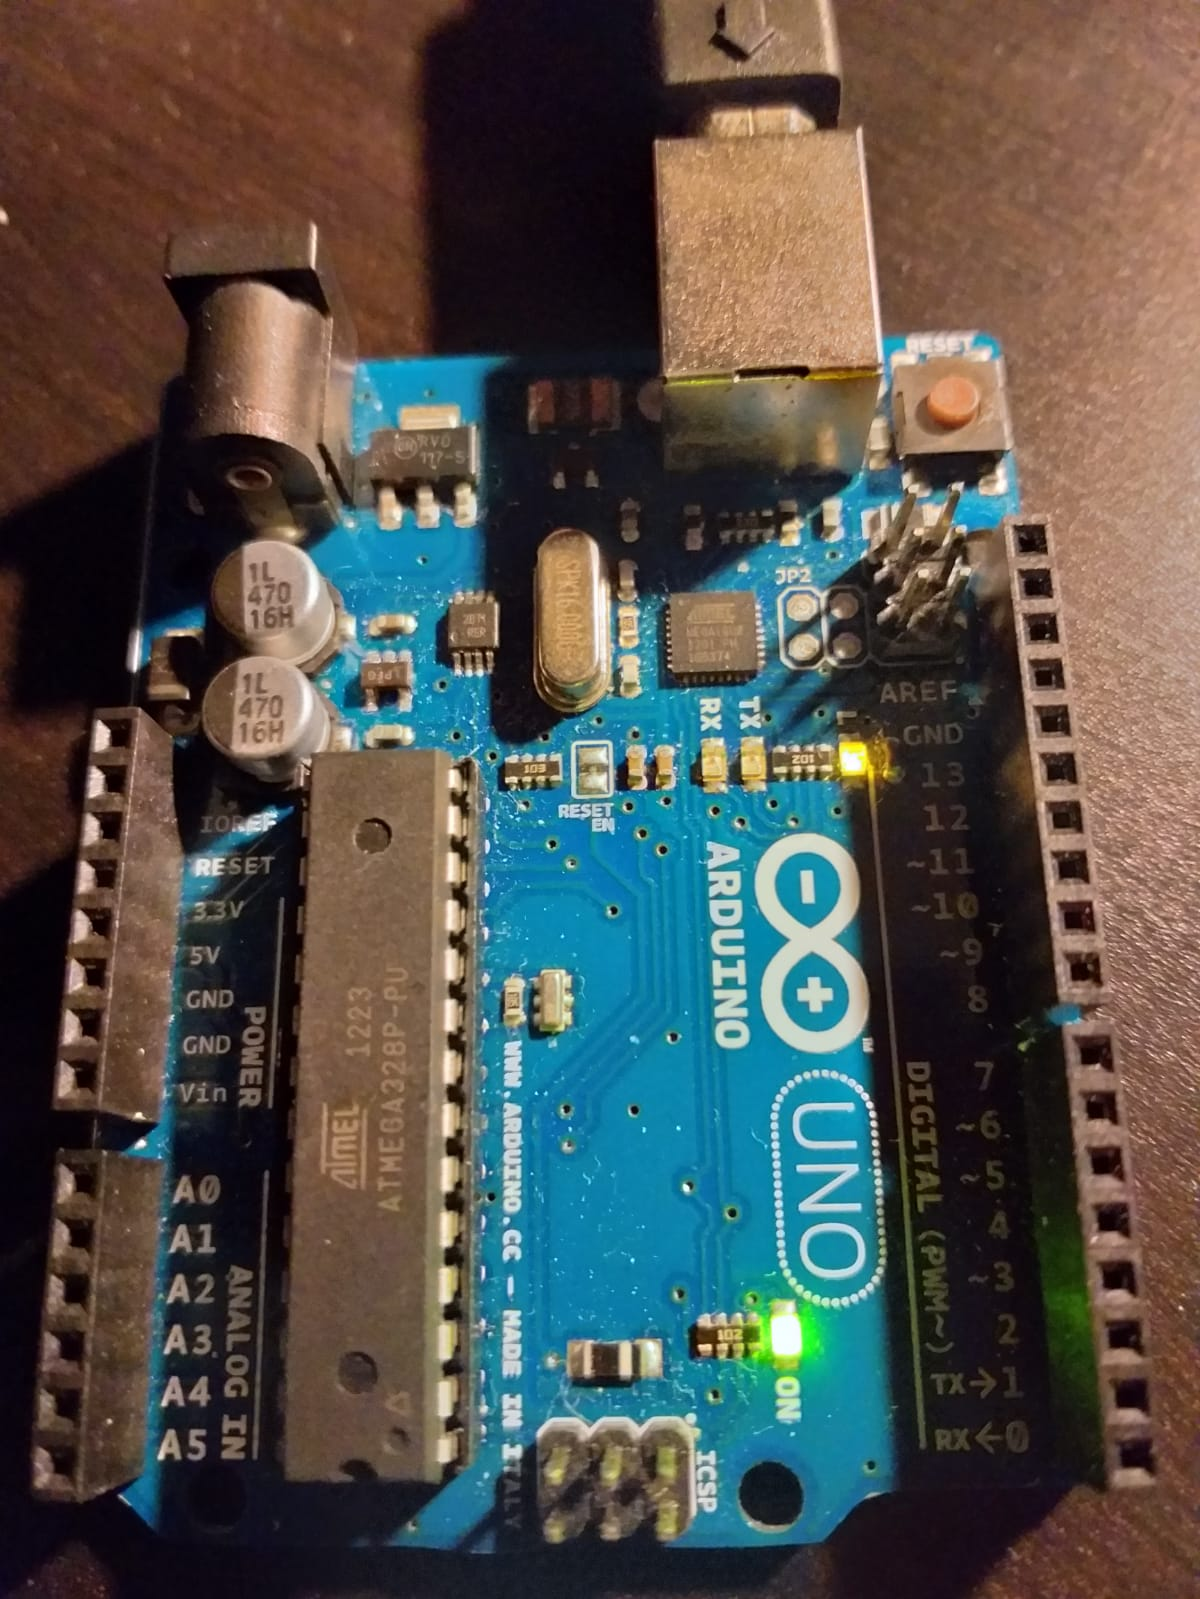
\includegraphics[width=0.75\textwidth]{arduino.jpeg}
		\caption{LED integrado de la placa \textit{Arduino} parpadeando}
	\end{figure}
	\bibliography{Report9}
\end{document}